% !TEX root = thesis.tex
\chapter{深層学習の実装における技術}
この章では、Deep Learningのアルゴリズムを実装して、実際の問題に適用するに当たって、どのようにすれば良い結果が得られるか、紹介する。
\section{評価基準}
Deep Learningのアルゴリズムを使用するための具体的な手段を選ぶにあたり、次のような判断基準を設けた。優先順位は、1→2→3の順に高い。
基準1. Deep Learningが注目された大きな理由である、高い識別精度を再現できる。
基準2. 学習にかかる時間が、他のアルゴリズムに比べて、極端に長くならない。
基準3. 利用にあたって必要なプログラミング量が出来るだけ少なく、バグが混入しにくい。
基準1は最優先目標である。今回Deep Learningを選択した理由は、Web工学のタスクにおいて、高い分類精度を実現するための最も有力な方法だと思われるからである。つまり、例えDeep Learningのアルゴリズムとして正しいプログラムだったとしても、分類精度が従来の分類器より劣っていれば意味はない。従来の分類器をそのまま使い続ければよいことになってしまう。
基準2と3は、現実の問題をDeep Learningで解決する際に、必要となってくる視点である。プログラムの作成や、学習の実行にかかる時間が、あまりにも長くなってしまうと、実際のビジネスや、刻一刻と変化するWebサービスに対して応用するのは非現実的だろう。
\section{既存ソースコード使用の利点}
Deep Learningのプログラムを実行するために、まず大きく分けて、「自分でソースコードを全て書く」方法と、「主に既存のソースコードを利用する」方法の2つが考えられる。今回は、既存ソースコードをベースに使うことを選択した。以下、その理由を説明する(図\ref{c4_library_merit}参考)。\par
「既存のソースコードを利用する」場合のメリットとして、「開発期間は基本的にゼロで済む」「新たにバグが混入する危険性が無い」「自分の改造コードが、他のライブラリ利用者によって使ってもらえるチャンスが大きい」という点が挙げられる。デメリットとして、「ソースコード中にブラックボックスが増え、改造にかかる時間が短くなる」「全く新しいアルゴリズムを実装する場合、ゼロからスタートした方が早く書けるケースもある」などが想定される。しかし、基準3の「プログラミング量が少なくバグのリスクが低い」という点において優れているため、今回は既存のソースコードを探して利用していくことにした。既存ソースコードを利用する際に生じるリスクについては、図\ref{c4_library_hedge}のように対処できる。\par

\begin{figure}[tbp]
 \begin{center}
  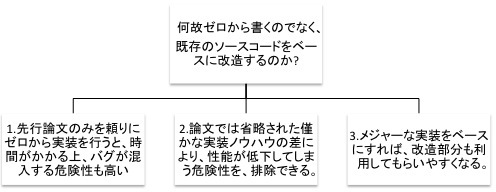
\includegraphics[width=100mm]{img/c4/library_merit}
 \end{center}
 \caption{既存コードの利用における、完全オリジナルコードの作成に対する利点}
 \label{c4_library_merit}
\end{figure}

\begin{figure}[tbp]
 \begin{center}
  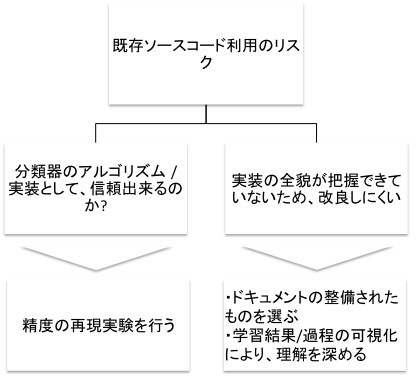
\includegraphics[width=120mm]{img/c4/library_hedge}
 \end{center}
 \caption{既存ソースコード利用のリスクと、対処方法}
 \label{c4_library_hedge}
\end{figure}

なお、「自分でソースコードを全て書く」場合のメリットとデメリットは、上記「既存のソースコード」の場合の逆となる。自分で新たなコードを書くので時間がかかり、バグの混入リスクも大きい。また、ソースコードを公開した場合の、ライブラリとしての信頼度も、ゼロから築かなければならない。ただし、コードの詳細部分を改造する段階では、自分の手で書いたコードを使う方が、より深い理解を得やすく、確実で素早い実装ができる可能性もある。\par

\section{Graphics Processing Unitの利用による高速化}
一般に、Deep Learningの研究においては、GPGPUによる並列計算が有効とされている。並列計算のプログラム構成にもよるが、100倍近く早くなることもある。また、Deep Learningの実装によっては、はじめからGPUで高速化することを前提に、GPU専用のコードを書いている場合があるこの場合、そもそもGPUを搭載したマシンを使わないと、コンパイルや実行が全く出来なくなってしまう。\\
CPUの計算能力は頭打ちになっている。GPUはmany coreによる高速演算ができる。NVIDIAはCUDAというGPUによる演算の開発環境を開発した。
\section{数値計算ライブラリTheanoの利点}
Theanoは、python上で記述される数式処理/数値計算ライブラリである。Theanoは、数式のコンパイルと実際のデータによる数値計算の2段階で動作する\cite{bergstra+al:2010-scipy}。図\ref{c4_theano_compile}に、Theanoが動作する仕組みを示した。
\begin{figure}[tbp]
 \centering
  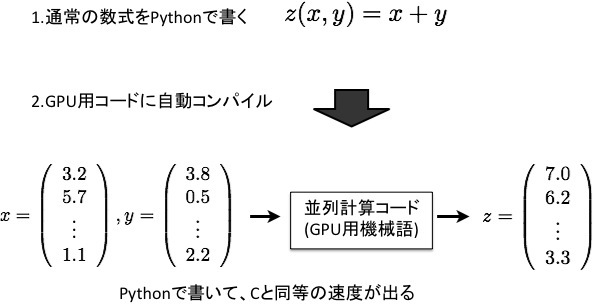
\includegraphics[width=100mm]{img/c4/theano_compile}
 \caption{Theanoの動作過程}
 \label{c4_theano_compile}
\end{figure}
Theanoでは、数式は文字シンボルを用いた文字式で記述される。このときデバッグの難しい数値計算の誤差絡みの部分、0divなど危険な処理を、自動的に解析してくれる。ニューラルネットワークの演算過程では、非常に小さい数値が出現することがあり、また、文字式を分析することで、計算グラフも最適化してくれる。プログラマは、プログラム上の些末な計算テクニックに囚われることなく、数式の本質的な部分の記述に集中することができる。また、微分も自動で行ってくれる。ニューラルネットワークでは、様々な文字の微分が必要になり、多層にすると爆発的に式が複雑になる。これを手計算による文字式の微分をしてから書いていくと、層を増やす度に手計算が必要になり、非常に煩雑で、開発効率が落ちてしまう。Theanoの自動微分と自動最適化は、pylearn2の内部記述の簡略化を大いに助けているおいて、多層のニューラルネットワークを使うときでも、文字式に対する大量の手計算と、大量のプログラムの式を書くことなく、簡単に微分やニューラルネットワークを拡張することができる。
\section{機械学習ライブラリPylearn2の利点}
今回は、Deep Learningを使うための既存ソースコードとして、モントリオール大学のLISA Lab.が提供している、pylearn2というライブラリを選んだ\cite{goodfellow2013pylearn2:}。pylearn2は、pythonで記述された、Deep Learningなど機械学習アルゴリズムを使うためのライブラリである。LISA Lab.を中心とする開発者によって、ソースコードの開発がほぼ毎日行われている。以下、pylearn2を選択した理由を記す。
\subsection{高精度アルゴリズムMaxout Networkの実装}
Pylearn2には、3章にて述べた、Maxout NetworkというDeep Learningのアルゴリズムの一種が実装されている。このアルゴリズムは、画像認識タスクにおいて非常に高い精度を実現しており、基準1を満たす上で都合が良い。
\subsection{Theanoの利用}
pylearn2のプログラムは、前述したTheanoを全面的に利用して記述されている。Theanoを用いたことで、可読性が大きく上昇している。また、何らかの理由で、pylearn2の部分的拡張が必要になったときでも、[過去のスライドを基に加筆]
\subsection{高度な拡張性と可読性}
pylearn2のソースコードは、拡張性や可読性を非常に強く意識して書かれている。基本的な使い方を記したチュートリアルのWebページが存在し、主なソースファイルには、詳細なドキュメントも記述されている。また、モジュール化が丁寧なので、自分で書く部分が少なくて済む。例えば、データセットを変更する場合は、Datasetクラスのみを書き下せばよく、他の部分に対してコードを書く必要がほとんどない。図\ref{c4_pylearn2_yaml}に、pylearn2において機械学習のアルゴリズムがどのようにモジュール化されているかを示す。\\
また、プログラムを改造する場合でも、数値パラメータを変更するだけであれば、設定ファイルのみの変更で完結させることができる。この設定ファイルは、YAML(YAML Ain't a Markup Language)形式に少し独自拡張を加えた形式になっている。\\
プログラム本体と、数値の設定ファイルが分離されていることで、プログラミングが不得手な人でも、比較的簡単に設定を変更することができる。\\
\begin{figure}[tbp]
 \begin{center}
  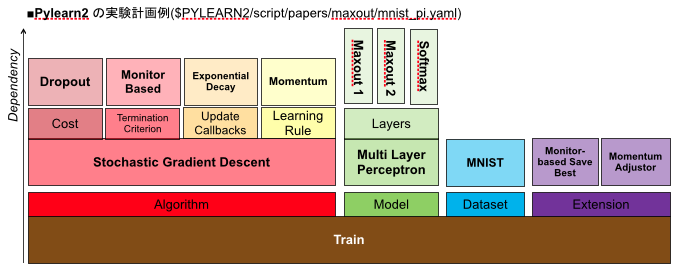
\includegraphics[width=80mm]{img/c4/pylearn2_yaml}
 \end{center}
 \caption{Pylearn2の実験計画例}
 \label{c4_pylearn2_yaml}
\end{figure}
\section{ハードウェアの構成}
pylearn2を通してDeep Learningのアルゴリズムを実行する、と決めたところで、実際にDeep Learningを利用するためのマシンを用意する必要がある。
まず、Deep Learningに限った話ではないが、機械学習のタスクは長時間の計算を必要とする場合が多く、プログラムの実行時間が1日以上かかることも稀ではない。普段使用しているPCが使えなくなると困る場合は、機械学習を動かしておくための専用サーバを用意することが望ましい。
GPUは必ずしも搭載していなくとも良いのだが、実践上TheanoやCUDAの性能を最大限に生かすためには、GPUを搭載しなければならない。また、CUDAを用いてGPUマシン専用に書かれたアルゴリズムを動作させるためには、GPUが必須となる。GPUは、NVIDIA製で、CUDAに対応していなければならない。ただし、グラフィック出力の機能はなくても構わない。2013年1月現在、NVIDIAのWebページに掲載されているGPUに関しては、全てCUDAに対応しているため、店舗で新品のGPUを購入する場合は基本的に問題は生じないと思われる。
NVIDIAのGPUの中で、どれを選ぶかも問題になる。NVIDIAのホームページでは、GPUのうちTeslaというシリーズがGPGPUに特化しており、非常に高精度/高速な演算を行うことができる、と述べられている。しかし、非常に高価な上、Teslaシリーズは一般的なグラフィックカードではなく、サーバ全体の購入を基本としている。販売員の方によれば、Teslaは主に商用の大規模データや、ミスの許されない長時間科学計算などに用いることを想定して作られている。今回の目的は、Web工学の一般的タスクにおけるDeep Learning技術を確立するという、いわば実験的な用途であり、Teslaの利用はオーバースペックだと思われる。
NVIDIAのGPUは、Teslaを除くと、QuadroとGeForceという2つのシリーズに分かれている。店舗の販売員の方に詳しい話を伺ったところ、Quadroはコンピュータグラフィックの出力機能に注力したシリーズであり、GeForceはより計算性能重視という傾向をもっている。つまり、Deep Learningの計算などGPGPUに用いる場合、同じ価格帯ならば、GeForceシリーズのGPUを用いた方が、費用対効果が大きくなると考えられる。
また、販売員の方によれば、GeForceシリーズの中でもTitanという機種は、Tesla用の部品の中で品質チェックに漏れてしまったものを流用しており、Teslaとほぼ同様の、非常に高い性能を発揮することが出来る、とのことだった。しかし、今回利用する中で最も計算量が大きいMaxout Networkについて、元の発表論文によれば、GeForceシリーズのGTX 580という、少し世代が前のGPUが用いられている。Deep Learningを実行させる上で、GPUが存在すること自体は非常に重要だが、必ずしも最新スペックのGPUが必要というわけではないことがわかる。
今回の構成では、知の構造化センターの中山浩太郎先生のアドバイスもあり、Titanではなく、同じGeForceシリーズのGTX 760というGPUを搭載することにした。
